\documentclass{article}
\usepackage[a4paper, total={6in, 8in}]{geometry}
\usepackage{algorithm}
\usepackage{algorithmic}
\usepackage{amsmath}
\usepackage{amssymb}
\usepackage{amsfonts}
\usepackage{bbm}
\usepackage{blindtext}
\usepackage{caption}
\usepackage{cancel}
\usepackage{color}
\usepackage{epstopdf}
\usepackage{etoolbox}
\usepackage{float}
\usepackage{graphicx}
\usepackage{hyperref}
\usepackage{multirow}
\usepackage{pgfplots}
\usepackage{tikz}
\usepackage{url}
\usepackage{times}
\usepackage{tkz-graph}
\usepackage[np]{numprint} 
\usepackage{verbatim}  
\usepackage{multicol}
\usepackage{threeparttable}
\usepackage{subcaption}
\usepackage{listings}
\usepackage{tkz-euclide}
\usepackage{stackengine}
\usepackage{enumitem}


\usetikzlibrary{calc}
\usetikzlibrary{fit}
\usetikzlibrary{arrows}
\usetikzlibrary{backgrounds}
\usetikzlibrary{shapes}
\usetikzlibrary{positioning}
\usetikzlibrary{decorations.pathmorphing}
\usetikzlibrary{decorations.pathreplacing}
\usetikzlibrary{decorations.markings}
\usetikzlibrary{arrows.meta}


\def\L{\mathcal{L}}
\def\E{\mathbb{E}}
\def\N{\mathcal{N}}
\def\KL{\mathbb{KL}}
\def\d{\text{d}}
\def\ep{{\epsilon}}
\def\VAR{\mathbb{VAR}}
\def\COV{\mathbb{COV}}

\def\a{{\mathbf a}}
\def\b{{\mathbf b}}
\def\c{{\mathbf c}}
%\def\d{{\mathbf d}}
\def\e{{\mathbf e}}
\def\f{{\mathbf f}}
\def\g{{\mathbf g}}
\def\h{{\mathbf h}}
\def\i{{\mathbf i}}
\def\j{{\mathbf j}}
\def\k{{\mathbf k}}
\def\l{{\mathbf l}}
\def\m{{\mathbf m}}
\def\n{{\mathbf n}}
\def\o{{\mathbf o}}
\def\p{{\mathbf p}}
\def\q{{\mathbf q}}
\def\r{{\mathbf r}}
\def\s{{\mathbf s}}
\def\t{{\mathbf t}}
\def\u{{\mathbf u}}
\def\v{{\mathbf v}}
\def\w{{\mathbf w}}
\def\x{{\mathbf x}}
\def\y{{\mathbf y}}
\def\z{{\mathbf z}}



\def\A{{\mathbf A}}
\def\B{{\mathbf B}}
\def\C{{\mathbf C}}
\def\D{{\mathbf D}}
%\def\E{{\mathbf E}}
\def\F{{\mathbf F}}
\def\G{{\mathbf G}}
\def\H{{\mathbf H}}
\def\I{{\mathbf I}}
\def\J{{\mathbf J}}
\def\K{{\mathbf K}}
%\def\L{{\mathbf L}}
\def\M{{\mathbf M}}
%\def\N{{\mathbf N}}
\def\O{{\mathbf O}}
\def\P{{\mathbf P}}
\def\Q{{\mathbf Q}}
\def\R{{\mathbf R}}
\def\S{{\mathbf S}}
\def\T{{\mathbf T}}
\def\U{{\mathbf U}}
\def\V{{\mathbf V}}
\def\W{{\mathbf W}}
\def\X{{\mathbf X}}
\def\Y{{\mathbf Y}}
\def\Z{{\mathbf Z}}

\def\0{{\bf 0}}
\def\1{{\mathbbm{1}}}
\def\Rad{\text{Rad}_n(\H)}
\def\RadE{\widehat{\text{Rad}}_S(\H)}
\def\RadF{\text{Rad}_n(\F)}
\def\aalpha{\boldsymbol{\alpha}}
\def\bbeta{\boldsymbol{\beta}}
\def\ggamma{\boldsymbol{\gamma}}
\def\eeta{\boldsymbol{\eta}}
\def\eepsilon{\boldsymbol{\epsilon}}
\def\llambda{\boldsymbol{\lambda}}
\def\ssigma{\boldsymbol{\sigma}}
\def\pphi{\boldsymbol{\phi}}
\def\ppi{\boldsymbol{\pi}}
\def\ppi{\boldsymbol{\mmu}}
\def\ttheta{\boldsymbol{\theta}}
\def\ddelta{\boldsymbol{\delta}}
\def\GGamma{{\boldsymbol{\Gamma}}}

\def\PR{{p_{\text{r}}}}
\def\PG{{p_{\text{g}}}}

\def\na{{\nabla}}

\newtheorem{definition}{Definition}
\newtheorem{theorem}{Theorem}
\newtheorem{lemma}{Lemma}
\newtheorem{proposition}{Proposition}
\newtheorem{conjecture}{Conjecture}
\newtheorem{example}{Example}
\newtheorem{property}{Property}
\newtheorem{comments}{Comments}
\newtheorem{remark}{Remark}


\DeclareMathOperator*{\argmin}{arg\,min}
\DeclareMathOperator*{\argmax}{arg\,max}

\def\delequal{\mathrel{\ensurestackMath{\stackon[1pt]{=}{\scriptstyle\Delta}}}}
\def\Dtheta{{\triangledown_\theta}}
\def\NT{{\nabla_\theta}}

\def\optional{{\color{red} Optional - not examinable}}

\def\exam{{\color{blue} High chance to be examined}}

\def\prox{{\text{prox}}}


\newlist{Properties}{enumerate}{2}
\setlist[Properties]{label=Property \arabic*., font=\textbf, itemindent=*}
\graphicspath{{images/}}

\usetikzlibrary{arrows}
\usetikzlibrary{fit,positioning}
\usetikzlibrary{arrows,shapes,positioning}
\usetikzlibrary{calc,decorations.markings}

\def\x{{\mathbf x}}
\def\X{{\mathbf X}}
\def\L{{\cal L}}
\def\C{\text{Const.}}
\def\E{\mathbb{E}}
\def\D{\text{d}}
\def\N{\mathcal{N}}
\def\KL{\text{KL}}
\def\U{\mathbf{U}}
\def\V{\mathbf{V}}
\def\u{\mathbf{u}}
\def\v{\mathbf{v}}
\def\d{\text{d}}
\def\a{\mathbf{a}}
\def\b{\mathbf{b}}
\def\w{\boldsymbol{w}}
\def\y{\boldsymbol{y}}
\def\H{\mathcal{H}}
\def\NT{{\nabla_\Theta}}
\def\BT{{\bf{\Theta}}}
\def\COV{{\mathbf{Cov}}}
%\def\SIGMA{{\boldsymbol {\Sigma }}}
\newcommand{\tens}[1]{%
  \mathbin{\mathop{\otimes}\limits_{#1}}%
}
\def\O{{\Theta}}
\def\GP{{\mathcal{GP}}}
\def\Var{{\text{Var}}}
\def\Cov{{\text{Cov}}}
%\def\ep{{\epsilon}}
\def\I{{\bf I}}
\def\f{{\bf f}}
\def\J{{\nabla_\Theta f}}
\def\A{{\mathcal{A}}}
\def\P{{{\Pr}}}
\def\1{{\mathbbm{1}}}
\def\Rad{\text{Rad}_n(\H)}
\def\RadE{\widehat{\text{Rad}}_S(\H)}
\def\tr{\text{tr}}
\def\V{{\mathbb{VAR}}}
\def\E{{\mathbb{E}}}
\def\D{\text{d}}
\def\S{{\mathbb{S}}}
\def\KL{{\text{KL}}}
\def\Y{{\bf Y}}
\def\X{{\bf X}}
\def\K{{\bf K}}
\def\A{{\bf A}}
\def\B{{\bf B}}
\def\P{{\bf P}}
\def\f{{\bf f}}
\def\tr{\text{Tr}}
\def\SIGMA{{\boldsymbol \Sigma}}
\def\MU{\boldsymbol {\mu }}


%\def\xp{x^{(p)}}
%\def\xpred{x^{({\color{red}p})}}
%\def\xq{x^{(q)}}
%\def\xqblue{x^{({\color{blue}q})}}


\def\xp{x}
\def\xpred{{\color{red}x}}
\def\xq{x'}
\def\xqblue{{\color{blue}x'}}


\def\din{{d_\text{in}}}
\def\T{{\Theta}}

\def\phiX{{\bar{a}(\dX)}}
\def\phix{{\bar{a}(x)}}
\def\K{{\mathcal{K}}}
\def\X{{\mathbf X}}
\def\R{{\mathcal R}}
\def\hyt{{\hat{y}_t}}
%\def\x{{\mathbf x}}
\def\dX{{\mathcal{X}}}
\def\Y{{\mathbf Y}}
\def\dY{{\mathcal{Y}}}
\def\ds{{| \mathcal{D} | }}
\def\delTh{{\triangle \Theta(t)}}
\def\flin{{f^{\text{lin}}_t}}
\def\flastl{{\hat{y}_t(x, \Theta^{L+1})}}
\def\fLastl{{\hat{y}_t(\dX, \Theta^{L+1})}}

\def\Rd{{\mathbb{R}}}
\def\xpd{{\bf x}}
\def\xqd{{\bf x}'}

\def\flin{{f^{\text{lin}}_t}}
\def\flind{{\dot{f}^{\text{lin}}_t}}
\def\dom{{\dot{\omega}}}
\def\fX0{{f_0(\dX, \Theta_0)}}
\def\fx0{{f_0(x, \Theta_0)}}
\def\EKAll{{\hat{\T}_0(\dX,\dX)}}
\def\dphi{{\dot{\phi}}}
\def\Apf{{\mathcal{A}_p(f)}}
\def\Aqf{{\mathcal{A}_q(f)}}

\def\QS{{\bf QUESTION }}
\def\OC{\color{white}}

\newcommand*\circled[1]{\tikz[baseline=(char.base)]{
            \node[shape=circle,draw,inner sep=2pt] (char) {#1};}}



% ── Paper-style layout (matches the transformer_standard_paper reference) ──────
\geometry{a4paper, textwidth=6.3in, textheight=9.2in}
\usepackage{fancyhdr}
\pagestyle{fancy}
\fancyhf{}
\fancyhead[L]{\small Expectation Maximization}
\fancyhead[R]{\small Richard Xu}
\fancyfoot[C]{\thepage}
\renewcommand{\headrulewidth}{0.4pt}
\setlength{\headheight}{14pt}

\title{\bfseries Expectation Maximization:\\
From Mixture Densities to a Provably\\
Convergent Algorithm}
\author{Richard Xu}
\date{}

\begin{document}

\maketitle
\thispagestyle{plain}

\begin{center}
\textit{Lecture notes and tutorial}
\end{center}

\begin{abstract}
\noindent
Data with several clusters cannot be described by a single Gaussian, and the
natural remedy --- a mixture of Gaussians --- produces a log-likelihood that
neither yields a closed-form maximum nor suits plain gradient ascent, since the
objective is non-concave. These notes develop the Expectation-Maximization
(E-M) algorithm as the standard answer. After reviewing convexity and Jensen's
inequality, we state the E-M update and prove its central guarantee: each
iteration leaves the log-likelihood non-decreasing. The proof is given twice
--- once through the ELBO--KL decomposition familiar from variational
inference, viewing E-M as maximization-maximization, and once directly through
the classical $Q$/$H$ decomposition, where a one-line Jensen argument shows the
cross-entropy term can never decrease. The framework is then applied in full to
the Gaussian Mixture Model: responsibilities form the E-step, and Lagrange
multipliers plus matrix calculus give closed-form M-step updates for the
mixing weights, means, and covariances, each a responsibility-weighted
average. A sanity check confirms the updates collapse to the single-Gaussian
maximum-likelihood estimates when $k=1$. Exercises with worked solutions
conclude the notes.
\end{abstract}

\vspace{2mm}
\noindent
\textbf{Keywords:} expectation maximization; Gaussian mixture model; latent
variables; Jensen's inequality; ELBO; maximum likelihood

\newpage
\tableofcontents
\newpage



\section{Motivation: Mixture Density Models}



When you have data that looks like:

\begin{figure}[H]
    \begin{center}
    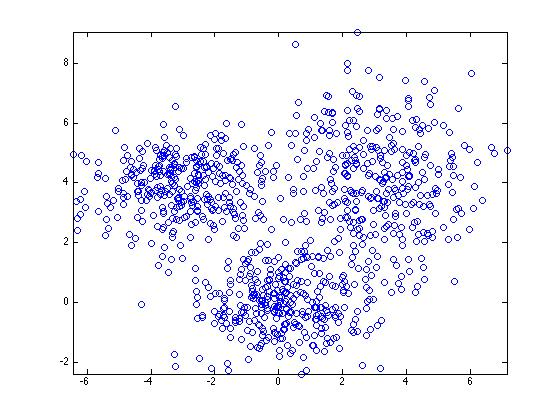
\includegraphics[scale=0.4]{gmm_data_3_mixtures.jpg}
     \end{center}
\end{figure}


%-------------------------------------------------------------



Can you fit them using a single-mode Gaussian distribution, i.e.,:

\begin{equation}
\begin{split}
p(x) &=  \mathcal{N}(x | \mu, \Sigma)\\
&=  (2 \pi)^{-k/2} | \Sigma |^{-\frac{1}{2}} \exp \Big( -\frac{1}{2} (x- \mu)^\top \Sigma^{-1} (x- \mu) \Big) \\
\end{split}
\end{equation}

Clearly not! Data like this is typically modelled using mixture densities \cite{bishop2006pattern} — in this case, a Gaussian Mixture Model with $k$ mixtures (GMM):

\begin{equation}\begin{split}
p(x) =  \sum_{l=1}^k \alpha_l \mathcal{N} (x | \mu_l, \Sigma_l) \quad\quad \text{s.t.}\quad \sum_{l=1}^k \alpha_l = 1
\end{split}\end{equation}











%-------------------------------------------------------------

\subsection{Gaussian Mixture model result}



\begin{figure}[H]
    \begin{center}
    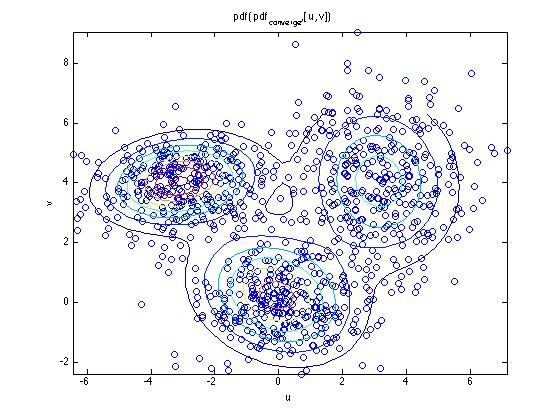
\includegraphics[scale=0.4]{gmm_result_3_mixtures.jpg}
     \end{center}
    \caption{GMM fitting result}
\end{figure}



%-------------------------------------------------------------




Let $\Theta = \{ \alpha_1, \dots \alpha_k, \mu_1, \dots \mu_k, \Sigma_1, \dots \Sigma_k \}$

\begin{equation}\begin{split}
\Theta_{\text{MLE}} &= \argmax_{\Theta} \L(\Theta |X)\\
 &=  \argmax_{\Theta} \bigg( \sum_{i=1}^n \log \sum_{l=1}^k \alpha_l \mathcal{N} (x_i | \mu_l, \Sigma_l) \bigg) \quad\quad \sum_{l=1}^k \alpha_l = 1
\end{split}\end{equation}

\begin{enumerate}
\item
Unlike the single-mode Gaussian, we cannot simply take derivatives and set them to zero, i.e., optimize it analytically.

\item
In terms of optimizing its parameters: the problem is {\bf non-concave}. So traditional gradient ascent is {\bf not} suitable for it, i.e., there are many local maxima.

\end{enumerate}

The {\bf goal} is to find an iterative process that ensures that $\log(p(X | \Theta^{(g)}))$ remains non-decreasing for $g = 1, \dots $. 

To do so, for data $X = \{x_1, \dots x_n\}$, we introduce ``latent'' variables $Z = \{ z_1, \dots z_n\}$, each $z_i$ indicating which mixture component $x_i$ belongs to. The core problem then simply boils down to fitting a single Gaussian.


\section{Preliminaries}

%-------------------------------------------------------------

\subsection{Convex function}

\begin{figure}[H]
    \begin{center}
    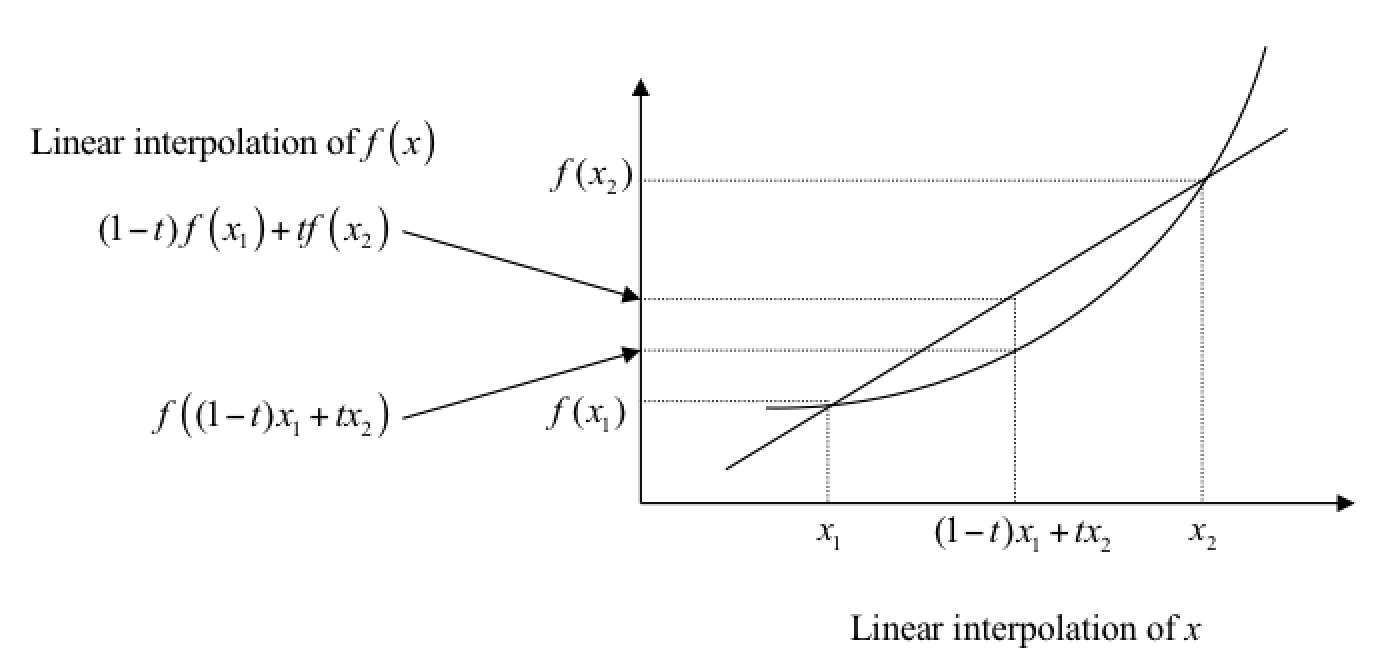
\includegraphics[scale=0.5]{convex.jpg}
     \end{center}
\end{figure}


\begin{equation}\begin{split}
f\left( (1-t) x_1 + t x_2 \right) \leq (1-t) f(x_1) + t  f(x_2)  \hspace{5 mm} t \in [0, 1]
\end{split}\end{equation}



%-------------------------------------------------------------

\subsection{Jensen’s inequality}


Using notation $\phi$ instead of $f$:

\begin{equation}\begin{split}
\phi \left( (1-t) x_1 + t x_2 \right) \leq (1-t) \phi (x_1) + t  \phi(x_2)  \hspace{5 mm} t \in [0, 1]
\end{split}\end{equation}

Can be generalized further for any convex combination, i.e., let $\sum_{i=1}^n p_i = 1$:

\begin{equation}\begin{split}
\phi \left( p_1 x_1 + p_2 x_2 + \dots + p_n x_n \right) &\leq p_1 \phi (x_1) + p_2  \phi(x_2) + \dots + p_n \phi (x_n)  \hspace{5 mm} \sum_{i=1}^n p_i = 1\\
\implies \phi \Big( \sum_{i=1}^n p_i x_i \Big) &\leq \sum_{i=1}^n p_i \phi (x_i) \\
\implies \phi \Big( \sum_{i=1}^n p_i f(x_i) \Big) &\leq \sum_{i=1}^n p_i \phi (f(x_i)) \hspace{5 mm} \text{ by replacing } x_i \text{ with } f(x_i)
\end{split}\end{equation}

generalize to the continuous case:

\begin{equation}\begin{split}
\phi \left( \int_{x } f(x) p(x) \d x \right) &\leq \int_{x }  \phi (f(x)) p(x) \d x \implies \phi \big( \E[  f(x) ] \big) \le \E [\phi (f(x))]
\end{split}\end{equation}




%-------------------------------------------------------------

\subsubsection{Jensen’s inequality example: $-\log(x)$}

$\phi(x) = -\log(x)$ is a convex function:


%\begin{figure}
%    \begin{center}
%    \includegraphics[scale=0.3]{minus_log.jpg}
%     \end{center}
%   \caption{plot of $\phi(x) = -\log(x)$}
%\end{figure}

\begin{figure}[H]
\begin{center}\label{fig:minus_log}
\begin{tikzpicture}[scale=0.7]
\begin{axis}[
    axis lines = left,
    xlabel = \(x\),
    ylabel = {\(-\log(x)\)},
]
\addplot [
    domain=0:5,
    samples=100,
    color=red,
]
{- ln(x)};
%\addplot[color=blue,thick] coordinates { (2.05,0) (2.05,0.243) };
%\addplot[color=red,thick] coordinates { (2.0,0) (2,0.073) };
\end{axis}
\end{tikzpicture}
\caption{example of convex function $-\log(x)$}
\end{center}
\end{figure}



%-------------------------------------------------------------

\begin{enumerate}
\item when $\phi(.)$ is convex:

\begin{equation}\begin{split}
 \phi  (\E[  f(\x) ]) &\le \E [\phi (f(\x))]\\
\text{e.g.}\quad  -\log ( \E[  f(\x) ] ) &\le \E [-\log (f(\x))]\\
\end{split}\end{equation}

\item when $\phi(.)$ is concave:


\begin{equation}\begin{split}
 \phi ( \E[  f(\x) ] ) &\ge \E [\phi (f(\x))]\\
\text{e.g.}\quad  \log ( \E[  f(\x) ] ) &\ge \E [ \log (f(\x))]\\
\end{split}\end{equation}

\end{enumerate}

%-------------------------------------------------------------

\section{Expectation-Maximization Algorithm}

Instead of performing:

\begin{equation}\begin{split}
\Theta^{\text{MLE}} &=  \argmax_{\Theta} \L(\Theta | X)\\ 
&= \argmax_{\Theta} \left(\log [p(X|\Theta)]  \right)  \\
\end{split}\end{equation}

{\bf The trick } is to introduce some ``latent'' variable $Z$ into the model.

For each iteration of the E-M algorithm \cite{dempster1977maximum}, we perform:

\begin{equation}\begin{split}
\Theta^{(g+1)} = \argmax_{\Theta} \left( \int_Z \log{(p(X,Z|\Theta))} p(Z|X,\Theta^{(g)}) \d Z \right)
\end{split}\end{equation}

However, before we apply it, we must ensure convergence \cite{wu1983convergence}, i.e.,

\begin{equation}\begin{split}
\log (p(X| \Theta^{(g+1)} )) &=  \L( \Theta^{(g+1)} | X)\\
&\ge \L( \Theta^{(g)} | X)\\
&= \log (p(X| \Theta^{(g)} )) \quad \forall g
\end{split}\end{equation}

Note the difference between the variable $\Theta$ and the constant $\Theta^{(g)}$. Also note that gradient ascent is {\bf not} suitable for many E-M problems, as they can be {\bf non-concave}.


%-------------------------------------------------------------

\section{Proof of convergence: Maximization-Maximization}

We have seen this in the variational-inference literature \cite{neal1998view}, as the ELBO-KL decomposition:

\begin{equation}\begin{split}
\L(\Theta|X) &= \log \left(p(X|\Theta) \right) \\
            &= \log \left( \frac{ p(X,Z|\Theta)}{ p(Z|X,\Theta) } \right) 
%= \log \left( \frac{ \frac{p(X,Z|\Theta)}{q(Z)}}{ \frac{ p(Z|X, \Theta)}{q(Z)} } \right) 
\\
            &= \log \left( \frac{p(X,Z|\Theta)}{q(Z)} \times \frac{ q(Z)}{p(Z|X,\Theta)} \right)\\
            &= \log \left(\frac{p(X,Z|\Theta)}{q(Z)} \right) + \log \left( \frac{q(Z)}{ p(Z|X,\Theta)} \right)\\
%\implies \log \left(p(X|\Theta) \right)
            &= \int_Z \log \left(\frac{p(X,Z|\Theta)}{q(Z)} \right)q(Z) \d Z + \int_Z \log \left( \frac{ q(Z)}{p(Z|X,\Theta)} \right)q(Z) \d Z\\
            &= \text{ELBO}(\Theta, q) + \KL \big( q(Z) \| p(Z|X,\Theta) \big) \\
%         &= F (\Theta, q ) + \int_Z \log \left( \frac{ q(Z)}{p(Z|X,\Theta)} \right)q(Z)\\
\end{split}\end{equation}



%-------------------------------------------------------------

%\subsection{Proof of convergence: using M-M (2)}
%Another way of knowing:
%\begin{equation}
%\begin{split}
%\mathcal{L}(\Theta|X) &= \log \left(p(X|\Theta) \right) \geq \int_Z \log \left(\frac{p(X,Z|\Theta)}{q(Z)} \right)q(Z)
%\end{split}
%\end{equation}

or to use Jensen's inequality:

\begin{equation}\begin{split}
\L(\Theta|X) 
&= \log p(X|\Theta) =  \log \int_Z  p(X, Z |\Theta) \d Z \\
&=\log \Big( \int_Z \frac{  p(X,Z|\Theta)}{q(Z)} q(Z) \d Z \Big)\\
&\ge  \int_Z \log \Big( \frac{  p(X,Z|\Theta)}{q(Z)} \Big) q(Z) \d Z \\
&= \text{ELBO}(\Theta, q)
\end{split}\end{equation}



%-------------------------------------------------------------

\subsection{Maximization of ELBO}

When applying E-M as a Maximization-Maximization algorithm, we only need to optimize ELBO, let's revisit the ELBO-KL decomposition again:


\begin{equation}\begin{split}\label{eq elbo kl decomposition}
\L(\Theta|X) &= \int_Z \log \left(\frac{p(X,Z|\Theta)}{q(Z)} \right)q(Z) \d Z + \int_Z \log \left( \frac{ q(Z)}{p(Z|X,\Theta)} \right)q(Z) \d Z\\
&= \text{ELBO} (\Theta, q ) + \KL ( q(Z) \| p(Z|X,\Theta) )\\
\end{split}\end{equation}

\begin{description}
\item [STEP 1:  fix $\Theta = \Theta^{(g)}$, maximize $q(Z)$ for ELBO] 
\end{description}

%\begin{itemize}
%\item $\L(\Theta | X)$ is fixed, i.e., indepedant of $q(Z)$. Therefore, $\L(\Theta | X)$ is the upper bound of $F (\Theta, q )$.
%\item  To make $\L(\Theta|X) = F (\Theta, q )$, i.e, $\KL(.) = 0$, we choose $q(Z) = p(Z|X,\Theta^{(g)})$. Therefore:
%\end{itemize}


\begin{equation}\begin{split}
q^* (\cdot)&= \argmax_{q} \{ \text{ELBO} (\Theta^{(g)}, q ) \}\\
&=\argmax_{q} \Big\{ \int_Z \log \left(\frac{p(X,Z|\Theta^{(g)})}{q(Z)} \right)q(Z) \d Z \Big\}\\
&= p(Z|X, \Theta^{(g)})\\
\implies \text{ELBO} (\Theta^{(g)}, q^* )  &= \L(\Theta^{(g)}|X)
\end{split}\end{equation}

This follows from the realization that when fixing $\Theta = \Theta^{(g)}$, the ELBO is upper-bounded by $\L(\Theta^{(g)} | X)$, and the maximum is attained exactly when $\KL(q^* \| p(Z|X, \Theta^{(g)} )) = 0$, i.e., $q^* = p(Z|X, \Theta^{(g)})$.

{\bf STEP 1} is invisible to the algorithm, but needs to be considered when interpreting convergence.


\begin{description}
      \item [STEP 2: fix  $q(\cdot) = p(Z|X, \Theta^{(g)})$, maximize $\Theta$]
\end{description}

substitute $q^* = p(Z|X, \Theta^{(g)} )$ back into the ELBO:


\begin{equation}\begin{split}\label{eq M-M update formula}
   \L(\Theta^{(g)}|X) &= \text{ELBO}(\Theta^{(g)}, q^*)\\
   &= \int_Z \log \left(\frac{p(X,Z|\Theta^{(g)})}{p(Z|X, \Theta^{(g)} )} \right) p(Z|X, \Theta^{(g)} ) \d Z\\
   &= \underbrace{\int_Z \log (p(X,Z|\Theta^{(g)})) p(Z|X, \Theta^{(g)} ) \d Z}_{Q (\Theta^{(g)} | \Theta^{(g)}) } \quad \underbrace{ - \int_Z \log (p(Z|X, \Theta^{(g)} )) p(Z|X, \Theta^{(g)} ) \d Z}_{H (\Theta^{(g)} | \Theta^{(g)}) }\\
\end{split}\end{equation}

It is obvious that, after computing the E-M update from the decomposition in Eq.(\ref{eq M-M update formula}), we have:

\begin{equation}\begin{split}\label{eq optimize Q}
\Theta^{(g+1)} &= \argmax_{\Theta} Q (\Theta | \Theta^{(g)})\\
&= \argmax_{\Theta} \Big( \int_Z \log{(p(X,Z|\Theta))} p(Z|X,\Theta^{(g)})  \d Z\Big)\\
\end{split}\end{equation}


then:

\begin{equation}\begin{split}
\underbrace{\int_Z \log (p(X,Z|\Theta^{(g+1)})) p(Z|X, \Theta^{(g)} ) \d Z}_{Q (\Theta^{(g+1)} | \Theta^{(g)}) } \ge \underbrace{\int_Z \log (p(X,Z|\Theta^{(g)})) p(Z|X, \Theta^{(g)} ) \d Z}_{Q (\Theta^{(g)} | \Theta^{(g)}) }
\end{split}\end{equation}

but if we can also prove:

\begin{equation}\begin{split}\label{eq show H is larger}
H(\Theta | \Theta^{(g)}) &\ge H(\Theta^{(g)} | \Theta^{(g)})\quad\quad \forall \Theta\\
\implies H(\Theta^{(g+1)} | \Theta^{(g)}) &\ge H(\Theta^{(g)} | \Theta^{(g)})
\end{split}\end{equation}

then we can show:

\begin{equation}\begin{split}
\L(\Theta^{(g+1)}|X) &= Q (\Theta^{(g+1)} | \Theta^{(g)}) + H (\Theta^{(g+1)} | \Theta^{(g)})\\
& \ge \underbrace{Q (\Theta^{(g)} | \Theta^{(g)})}_{\text{Eq.(\ref{eq optimize Q})}} + \underbrace{H (\Theta^{(g)} | \Theta^{(g)})}_{\text{Eq.(\ref{eq show H is larger})}}\\
& = \L(\Theta^{(g)}|X)\\
\end{split}\end{equation}


Note that since $Q (\Theta | \Theta^{(g)}) + H (\Theta | \Theta^{(g)}) = \L(\Theta|X)$ identically, jointly maximizing both terms would recover the (intractable) MLE itself. E-M maximizes only $Q$, so in general:

\begin{equation}\begin{split}
\bar{\Theta} &= \argmax_{\Theta} \big\{ Q (\Theta | \Theta^{(g)}) + H (\Theta | \Theta^{(g)}) \big\}\\
\implies \L(\Theta^{(g+1)}) &\le \L(\bar{\Theta}) \\
\end{split}\end{equation}


\subsubsection{why $H(\Theta | \Theta^{(g)}) \ge  H(\Theta^{(g)} | \Theta^{(g)})\quad\quad \forall \Theta$}

\begin{enumerate}
\item cross entropy

\begin{equation}\begin{split}
H(\Theta | \Theta^{(g)}) &= -  \int_{Z } \log (p(Z|X,\Theta)) p(Z|X,\Theta^{(g)}) \d Z\\
&= \text{Cross-Entropy} \big(p(Z|X,\Theta^{(g)}) \|  p(Z|X,\Theta) \big)\\
\implies \argmin_{\Theta} \{ H(\Theta | \Theta^{(g)}) \} &= \Theta^{(g)}\\
\implies \min_{\Theta} \{ H(\Theta | \Theta^{(g)}) \} &= \text{Entropy}( p(Z|X,\Theta^{(g)}))\\
\end{split}\end{equation}

\item directly

\begin{equation}\begin{split} 
&H( \Theta | \Theta^{(g)}) - H(\Theta^{(g)} | \Theta^{(g)})\\
&= \int_{Z } - \log (p(Z|X,\Theta)) p(Z|X,\Theta^{(g)}) \d Z - \int_{Z }  -\log \big( p(Z|X,\Theta^{(g)}) \big) p(Z|X,\Theta^{(g)}) \d Z \\
%------------------------------
&= \int_{Z }  \log \left( \frac{p(Z|X,\Theta^{(g)})}{p(Z|X,\Theta)} \right) p(Z|X,\Theta^{(g)}) \d Z\\
%&= \E_{Z \sim p(Z|X,\Theta^{(g)}) } \Big[ \log \Big( \frac{p(Z|X,\Theta^{(g)})}{p(Z|X,\Theta)} \Big) \Big]\\
&= \int_{Z }  - \log \left( \frac{p(Z|X,\Theta)}{p(Z|X,\Theta^{(g)})} \right) p(Z|X,\Theta^{(g)}) \d Z\\
&\ge   - \log \left( \int_{Z} \frac{p(Z|X,\Theta)}{p(Z|X,\Theta^{(g)})} p(Z|X,\Theta^{(g)}) \d Z \right)\\ 
&= 0\quad \because \phi = - \log \text{ is a convex function}
\end{split}\end{equation}


\end{enumerate}


% after obtaining $\Theta^{(g+1)}$, it will introduce a new likelihood function $\L(\Theta^{(g+1)} | X)$ for which the upper bound of the $\text{ELBO}(\Theta^{(g+1)}, q)$ is increased for {\bf STEP 1}



%diagrammatically, this can be represented as:
%\begin{enumerate}
%\item $\L(\Theta^{(g)}) = \text{ELBO}(\Theta^{(g)}, q) + \KL(q, p(Z | X, \Theta^{(g)}) )$
%\end{enumerate}


%\subsubsection{reason to update Eq.(\ref{eq M-M update formula}) only}
%We don't need to maximize any terms involving $\log(q(Z))q(Z)$, therefore the remaining terms becomes:
%\begin{equation}\begin{split}
%\Theta^*&= \argmax_{\Theta} \Big\{ \int_Z \log p(X,Z|\Theta) p(Z|X, \Theta^{(g)}) - \int_Z \log p(Z|X, \Theta) p(Z | X, \Theta^{(g)}) \Big\}\\
%&= \argmax_{\Theta} \Big\{ \int_Z \log p(X,Z|\Theta) p(Z|X, \Theta^{(g)}) + \text{CE}\big( p(Z | X, \Theta^{(g)}) \; \| \; p(Z|X, \Theta) \big)  \Big\}\\
%\end{split}\end{equation}
%Since we would like to have:
%\begin{equation}\begin{split}\label{eq M-M convergence}
%\L(\Theta^{(g+1)}|X) \ge \L(\Theta^{(g)}|X)  \quad\quad \forall g \ge 1
%\end{split}\end{equation}
%we know that:
%\begin{equation}\begin{split}
%\text{CE}\big( p(Z | X, \Theta^{(g)}) \; \| \; p(Z|X, \Theta^{(g)}) \big) &= 0\\
%\implies \text{CE}\big( p(Z | X, \Theta^{(g)}) \; \| \; p(Z|X, {\color{red}\Theta} \big) &\ge \text{CE}\big( p(Z | X, \Theta^{(g)}) \; \| \; p(Z|X, \Theta^{(g)}) \big) \quad \forall  {\color{red}\Theta} \\
%\end{split}\end{equation}
%Therefore, as long as we can optimize E-M (or M-M) of the part in Eq.(\ref{eq M-M update formula}), then we can ensure convergence as per Eq.(\ref{eq M-M convergence}).


\subsection{Proof of convergence without ELBO}

let's decompose $\L(\Theta|X)$ into:

\begin{equation}\begin{split}
\L(\Theta|X) &= \log (p(X |\Theta))\\
&= \log (p(Z,X|\Theta) ) -  \log ( p(Z|X,\Theta) )\\
% \implies&  \int_{Z} \log (p(X |\Theta)) p(Z|X,\Theta^{(g)}) \d Z\\
\end{split}\end{equation}

take the expectation of both sides with respect to $ p(Z|X,\Theta^{(g)}) $:

\begin{equation}\begin{split}\label{eq historical E-M formula}
\L(\Theta|X) &= 
\underbrace{\int_{Z } \log (p(Z,X|\Theta)) p(Z|X,\Theta^{(g)}) \d Z}_{Q ( \Theta | \Theta^{(g)}) } \; \underbrace{-  \int_{Z } \log (p(Z|X,\Theta)) p(Z|X,\Theta^{(g)}) \d Z}_{H (\Theta | \Theta^{(g)})}\\
\implies \L(\Theta^{(g)}|X) &=
\underbrace{\int_{Z } \log (p(Z,X|\Theta^{(g)})) p(Z|X,\Theta^{(g)}) \d Z}_{Q ( \Theta^{(g)} | \Theta^{(g)}) } \; \underbrace{-  \int_{Z } \log (p(Z|X,\Theta^{(g)})) p(Z|X,\Theta^{(g)}) \d Z}_{H (\Theta^{(g)} | \Theta^{(g)})}\\
\end{split}\end{equation}

where $H (\Theta | \Theta^{(g)}) = \text{Cross-Entropy} \big(p(Z|X,\Theta^{(g)}) \|  p(Z|X,\Theta) \big)$. 

\vspace{2mm}

Eq.(\ref{eq historical E-M formula}) can be considered as a simpler version of the ELBO-KL decomposition of $\L(\Theta | X)$ we have seen previously in Eq.(\ref{eq M-M update formula}).


% \begin{equation}\begin{split}
% \L(\Theta|X) &= 
% \int_{Z } \log \Big(\frac{p(Z,X| \Theta)}{p(Z|X,\Theta^{(g)})}\Big) p(Z|X,\Theta^{(g)}) \d Z \; -  \int_{Z } \log \Big(\frac{p(Z|X,\Theta)}{p(Z|X,\Theta^{(g)})}\Big) p(Z|X,\Theta^{(g)}) \d Z\\
% \end{split}\end{equation}

% i.e., the added term $\log \big( p(Z|X,\Theta^{(g)})\big) p(Z|X,\Theta^{(g)}) $ of the two terms cancel out and equivalent to Eq.(\ref{eq historical E-M formula}).

% \subsubsection{why only $Q ( \Theta | \Theta^{(g)})$ needs to be maximized}


% In E-M, we only maximize non $\Theta$ part of ELBO:



% instead of maximizing the entire Eq.(\ref{eq historical E-M formula}), i.e., $Q (\Theta | \Theta^{(g)}) + H (\Theta | \Theta^{(g)})$

% \hspace{2mm}



%and:
%\begin{equation}\begin{split}
%\L(\Theta^{(g+1)} | X) - \L(\Theta^{(g)} | X) \le \L(\bar{\Theta}| X) - \L(\Theta^{(g)} | X)
%\end{split}\end{equation}

%however, it will not matter, as $\Theta^{(g+1)}$ is obtained using an easier formulation and won't matter if it converge a bit slower.

%\begin{equation}\begin{split}
%\argmax_{\Theta} \left[ \int_{Z }  \log (p(Z|X,\Theta)) p(Z|X,\Theta^{(g)}) \d Z \right]  = \Theta^{(g)} 
%\implies H(\Theta^{(g+1)}, \Theta^{(g)}) \leq H(\Theta^{(g)}, \Theta^{(g)}) 
%\end{split}\end{equation}
%Then 
%\begin{equation}\begin{split}
%\L(\Theta^{(g+1)} = \underbrace{q(\Theta^{(g+1)}, \Theta^{(g)})}_{\geq q(\Theta^{(g)}, \Theta^{(g)})} - \underbrace{H(\Theta^{(g+1)}, \Theta^{(g)})}_{\leq H(\Theta^{(g)}, \Theta^{(g)})}  \geq q(\Theta^{(g)}, \Theta^{(g)}) - H(\Theta^{(g)}, \Theta^{(g)}) = \L(\Theta^{(g)}
%\end{split}\end{equation}




%-------------------------------------------------------------


%\begin{equation}\begin{split}
%&\text{To prove} \hspace{5 mm} \argmax_{\Theta} [H(\Theta, \Theta^{(g)})] =  \argmax_{\Theta} \left[ \int_{z }  \log (p(Z|X,\Theta)) p(z|X,\Theta^{(g)}) \d z \right]  = \Theta^{(g)}\\
%\implies &\text{To prove} \hspace{5 mm} H(\Theta^{(g)}, \Theta^{(g)}) - H(\Theta, \Theta^{(g)}) \geq 0 \hspace{2 mm} \forall \Theta
%\end{split}\end{equation}





 




%-------------------------------------------------------------

%\subsection{The E-M Examples }
%
%\begin{itemize}
%\item Gaussian Mixture Model
%\item Probabilistic Latent Semantic Analysis (PLSA)
%\end{itemize}





%-------------------------------------------------------------

%\subsection{The E-M Examples: Probabilistic Latent Semantic Analysis (PLSA) (1)}
%%    \usetikzlibrary{arrows,%
%%                shapes,positioning}
%    \begin{tikzpicture}[>=latex]
%      \tikzset{node distance = 3cm}
%      \tikzset{VertexStyle/.style  = {shape         = circle,
%                                      draw          = black,
%                                      inner sep     = 2pt,%
%                                      minimum size  = 8mm,
%                                      outer sep     = 0pt,
%                                      fill          = gray!50}}
%      \node[VertexStyle](D){D};
%      \node[VertexStyle,right=3 cm of D](Z){Z};
%      \node[VertexStyle,right=3 cm of Z](W){W};
%      \tikzset{LabelStyle/.style = {fill=white}}
%      \tikzset{EdgeStyle/.style  = {->}}
%      \Edge[label=$P(z_k|d_i)$](D)(Z)
%      \Edge[label=$P(w_j|z_k)$](Z)(W)
%    \end{tikzpicture}
%
%\begin{itemize}
%\item $D = \{ d_1, \dots, d_N \}$ are articles, $Z = \{z_1, \dots, z_k \}$ are topics, $W = \{ w_1, \dots, w_M \}$ are words
%\item $P(z_k|d_i) \sim \text{Mult}({\bf P_1})$  and $P(w_j|z_k) \sim \text{Mult}({\bf P_2})$
%\item There are $N \times K$ different ${\bf P_1}$  and $M \times K$ different ${\bf P_1}$ \\
%	Therefore, we refer $P(z_k|d_i)$ and $P(w_j|z_k)$ as parameters $\Theta$
%\item Obviously, direct maximization don't work!
%\end{itemize}
%
%    
%
%
%%-------------------------------------------------------------
%
%
%\subsection{The E-M Examples: Probabilistic Latent Semantic Analysis (PLSA) (2) }
%
%\begin{itemize}
%\item  $n(d_i,w_j)$ is the number of words $w_j$ appear in the document $d_i$, and they should have {\bf same } probability:
%\end{itemize}
%
%	\begin{equation}
%            \Pr (D, W, Z = z_k | \Theta ) \propto \Pr (W | z_k) \Pr (z_k | D) = \prod_{i=1}^{N} \prod_{j=1}^{M}  \left[ \Pr(w_j | z_k) \Pr( z_k | d_i) \right]^{n(d_i,w_j)}
%	\end{equation}
%
%and
%
%	\begin{equation}
%	\begin{split} 
%            P(z_k|d_i,w_j) =\frac{P(d_i,w_j|z_k)P(z_k)}{\sum_{l=1}^{K} P(d_i,w_j|z_l)P(z_l)} 
%		\\
%=\frac{P(w_j|z_k)P(z_k|d_i)}{\sum_{l=1}^{K} P(w_j|z_l)P(z_l|d_i)}
%	\end{split}
%	\end{equation}
%
%
%
%%-------------------------------------------------------------
%
%
%\subsection{The E-M Examples: Probabilistic Latent Semantic Analysis (PLSA) (2) }
%
%Substitube into E-M:
%
%\begin{equation}
%\begin{split}
%q( \Theta, \Theta^{(g)}) &= \int_z \log{(p(X,Z|\Theta))} p(Z|X,\Theta^{(g)}) \d z\\
%&= \sum_{k=1}^K \log{ \left( \prod_{i=1}^{N} \prod_{j=1}^{M}  \left[ \Pr(w_j | z_k) \Pr( z_k | d_i) \right]^{n(d_i,w_j)}\right)} \Pr (z_k | W, D , \Theta^{(g)})\\
%&= \sum_{k=1}^K  \sum_{i=1}^{N} \sum_{j=1}^{M}  n(d_i,w_j) \log \left[ \Pr(w_j | z_k) \Pr( z_k | d_i) \right] \Pr (z_k | W, D , \Theta^{(g)})\\
%&= \sum_{i=1}^{N} \sum_{j=1}^{M}  n(d_i,w_j) \sum_{k=1}^K  \log \left[ \Pr(w_j | z_k) \Pr( z_k | d_i) \right] \Pr (z_k | W, D , \Theta^{(g)})
%\end{split}
%\end{equation}
%
%
%
%
%%-------------------------------------------------------------
%
%\subsection{The E-M Examples: Probabilistic Latent Semantic Analysis (PLSA) }
%
%    The latent variables' posterior probability is,
%        \begin{eqnarray*}
%            P(z_k|d_i,w_j)=\frac{P(d_i,w_j|z_k)P(z_k)}{\sum_{l=1}^{K} P(d_i,w_j|z_l)P(z_l)}=\frac{P(w_j|z_k)P(z_k|d_i)}{\sum_{l=1}^{K} P(w_j|z_l)P(z_l|d_i)}
%        \end{eqnarray*}
%       
%  \begin{eqnarray*}
%            L_c(\Theta)&=& \sum\nolimits_{i=1}^{N} \sum\nolimits_{j=1}^{M} n(d_i,w_j) log \prod_{k=1}^{K} (P(z_k|d_i)P(w_j|z_k))^{z_k}
%            \\
%            &=& \sum\nolimits_{i=1}^{N} \sum\nolimits_{j=1}^{M} n(d_i,w_j) \sum_{k=1}^{K} z_k log  (P(z_k|d_i)P(w_j|z_k))
%        \end{eqnarray*}
%        As a result,
%        \begin{eqnarray*}
%            q(\Theta ; \Theta^{n}) &=& \sum_{k=1}^{K} L_c(\Theta) P(z_k|D,W)
%            \\
%             &=& \sum\nolimits_{i=1}^{N} \sum\nolimits_{j=1}^{M} n(d_i,w_j) \sum_{k=1}^{K} P(z_k|d_i,w_j) log  \left(P(z_k|d_i)P(w_j|z_k)\right)
%        \end{eqnarray*}
%
%
%
%
%
%
%
%%-------------------------------------------------------------
%
%\subsection{The E-M Examples: Probabilistic Latent Semantic Analysis (PLSA) }
%
%
%\begin{equation}
%\begin{split}
%            \mathbb{LM}(\Theta,\tau,\rho) &= q(\Theta, \Theta^{(g)})+\sum_{k=1}^{K}\tau_{k} \left( 1-\sum_{j=1}^{M}P(w_j|z_k) \right) + \sum_{i=1}^{N} \rho_{i}\left( 1-\sum_{k=1}^{K}P(z_k|d_i)\right)\\
%	&=  \sum_{i=1}^{N} \sum_{j=1}^{M}  n(d_i,w_j) \sum_{k=1}^K  \log \left[ \Pr(w_j | z_k) \Pr( z_k | d_i) \right] \Pr (z_k | W, D , \Theta^{(g)})\\
%&\hspace{10 mm} + \sum_{k=1}^{K}\tau_{k} \left( 1-\sum_{j=1}^{M}P(w_j|z_k) \right) + \sum_{i=1}^{N} \rho_{i}\left( 1-\sum_{k=1}^{K}P(z_k|d_i)\right)\\
%\end{split}
%\end{equation}
%
%\begin{equation}
%\begin{split}
% \frac{\partial \mathbb{LM}(\Theta,\tau,\rho)}{\partial P(z_k|d_i)} &= \sum_{j=1}^{M}  n(d_i,w_j)   \frac{\Pr(w_j | z_k)}{\Pr( z_k | d_i)} \Pr (z_k | W, D , \Theta^{(g)})= 0\\
%\implies &\sum_{j=1}^{M}  n(d_i,w_j)  \Pr(w_j | z_k)  \Pr (z_k | W, D , \Theta^{(g)}) + \Pr( z_k | d_i) (n+1) \sum_{i=1}^{N} \rho_{i} = 0
%\end{split}
%\end{equation}
%
%        And then , we get four equations.
%        \begin{eqnarray*}
%        \frac{\partial \mathbb{LM}(\Theta,\tau,\rho)}{\partial P(z_k|d_i)} &=& 0
%        \\
%        \frac{\partial LM(\Theta,\tau,\rho)}{\partial P(w_j|z_k)} &=& 0
%        \\
%        \sum_{k=1}^{K} P(z_k|d_i) &=&1
%        \\
%        \sum_{j=1}^{M} P(w_j|z_k) &=&1
%        \end{eqnarray*}
%
%
%
%%-------------------------------------------------------------
%
%\subsection{The E-M Examples: Probabilistic Latent Semantic Analysis (PLSA) }
%
%
%
%        We simplify these four equations.
%        \begin{eqnarray*}
%        \sum_{i=1}^{N}n(d_i,w_j)P(z_k|d_i,w_j)-\tau_{k}P(w_j|z_k) &=& 0
%        \\
%        \sum_{j=1}^{M}n(d_i,w_j)P(z_k|d_i,w_j)-\rho_{i}P(z_k|d_i) &=& 0
%        \\
%        \sum_{k=1}^{K} P(z_k|d_i) &=&1
%        \\
%        \sum_{j=1}^{M} P(w_j|z_k) &=&1
%        \end{eqnarray*}
%        And then we get the result.
%        \begin{eqnarray*}
%        P(w_j|z_k)&=&\frac{\sum_{i=1}^{N}n(d_i,w_j)P(z_k|d_i,w_j)}{\sum_{m=1}^{M}\sum_{i=1}^{N}n(d_i,w_m)P(z_k|d_i,w_m)}
%        \\
%        P(z_k|d_i)&=&\frac{\sum_{j=1}^{M}n(d_i,w_j)P(z_k|d_i,w_j)}{n(d_i)}
%        \\
%        \tau_{k}&=&\sum_{m=1}^{M}\sum_{i=1}^{N}n(d_i,w_m)P(z_k|d_i,w_m)
%        \\
%        \rho_{i}&=&n(d_i)
%        \end{eqnarray*}
%
%

%-------------------------------------------------------------
\newpage

\section{E-M Example: Gaussian Mixture Model}

Gaussian Mixture Model (k-mixture) (GMM):

\begin{equation}
\begin{split}
p(x|\Theta) =  \sum_{l=1}^k \alpha_l \mathcal{N} (x | \mu_l, \Sigma_l) \hspace{5 mm} \sum_{l=1}^k \alpha_l = 1\\
\text{ and } \Theta = \{ \alpha_1, \dots \alpha_k, \mu_1, \dots \mu_k, \Sigma_1, \dots \Sigma_k \}\\
\end{split}
\end{equation}


For data $X = \{x_1, \dots x_n\}$ we introduce ``latent'' variables $Z = \{ z_1, \dots z_n\}$, where each $z_i$ indicates which mixture component $x_i$ belongs to.

Looking at the E-M algorithm:

\begin{equation}
\begin{split}
\Theta^{(g+1)} = \argmax_{\Theta} \left[ q(\Theta, \Theta^{(g)}) \right]= \argmax_{\Theta} \left( \int_Z \log{(p(X,Z|\Theta))} p(Z|X,\Theta^{(g)}) \d Z \right)
\end{split}
\end{equation}

All we need to do is to define both $p(X,Z|\Theta)$ and $p(Z|X,\Theta)$ 



%-------------------------------------------------------------

\subsection{Gaussian Mixture Model in action}


\begin{equation}
\begin{split}
p(X|\Theta) =  \prod_{i=1}^n p(x_i|\Theta) = \prod_{i=1}^n \sum_{l=1}^k \alpha_l \mathcal{N} (x_i | \mu_l, \Sigma_l)
\end{split}
\end{equation}

{\bf How to define $p(X,Z|\Theta)$}  

\begin{equation}
\begin{split}
p(X,Z|\Theta) &= \prod_{i=1}^{n} p(x_i, z_i | \Theta) = \prod_{i=1}^{n} \underbrace{p(x_i | z_i , \Theta)}_{\mathcal{N}(x_i | \mu_{z_i}, \Sigma_{z_i} )} \underbrace{p ( z_i | \Theta)}_{\alpha_{z_i}}
= \prod_{i=1}^{n} \alpha_{z_i} \mathcal{N}(x_i | \mu_{z_i}, \Sigma_{z_i} )\\
\end{split}
\end{equation}

Notice that $p(X,Z|\Theta)$ is actually simpler than $p(X|\Theta)$.

\vspace{5 mm}

{\bf How to define $p(Z|X,\Theta)$}  

\begin{equation}
\begin{split}
p(Z|X,\Theta) &= \prod_{i=1}^{n} p(z_i | x_i , \Theta) = \prod_{i=1}^{n} \frac{\alpha_{z_i} \mathcal{N}(x_i | \mu_{z_i}, \Sigma_{z_i} )}{\sum_{l=1}^k \alpha_{l} \mathcal{N}(x_i | \mu_{l}, \Sigma_{l} )}\\
\end{split}
\end{equation}



%-------------------------------------------------------------

\subsection{The E-Step}


\begin{equation}\begin{split}
q(\Theta, \Theta^{(g)}) &=  \int_Z \log{(p(X,Z|\Theta))} p(Z|X,\Theta^{(g)}) \d Z \\
&=  \int_{z_1} \dots \int_{z_n} \left( \sum_{i=1}^{n} \log p(z_i ,  x_i | \Theta) \prod_{i=1}^n p(z_i|x_i,\Theta^{(g)}) \right) \d z_1 \cdots \d z_n \\
\end{split}\end{equation}




%-------------------------------------------------------------

\subsection{Some derivation to help}


let $p(Y)$ be the joint pdf $p(y_1,\dots y_N)$, and let $F(Y)$ be an additively separable function, where each term involves only one variable $y_i$, i.e.,

\begin{equation}\begin{split}
F(Y) = f_1(y_1) + \dots + f_N (y_N) = \sum_{i=1}^N f_i(y_i)
\end{split}\end{equation}


then,

\begin{equation}\begin{split}\label{eq integral of sum to sum of integral}
\int_{y_1} \dots \int_{y_N}  \Big(\sum_{i=1}^N f_i(y_i)\Big) p(Y) \d Y = \sum^N_{i=1} \bigg(  \int_{y_i} f_i(y_i) p(y_i) \d y_i \bigg)
\end{split}\end{equation}


%-------------------------------------------------------------

\subsubsection{Proof}

\begin{equation}
\int_Y F(Y) p(Y) \d Y = \int_{y_1} \int_{y_2}\dots \int_{y_N}  \Big(   \sum_{i=1}^N f_i(y_i) \Big) p(Y) \d y_1 \cdots \d y_N
\end{equation}

Expanding it out, this equation has $N$ sum terms:

\begin{equation}\begin{split}
&= \int\limits_{y_1} \int\limits_{y_2} \dots \int\limits_{y_N}  {\color{red} f_1(y_1)} p(y_1,\dots,y_N) \prod_{i=1}^N \big( \d y_i \big)
+ \dots + \int\limits_{y_1} \int\limits_{y_2} \dots \int\limits_{y_N}  {\color{red}f_N(y_N)} p(y_1,\dots,y_N) \prod_{i=1}^N \big( \d y_i \big)\\ 
&= \int\limits_{y_1} {\color{red} f_1(y_1) \d y_1} \bigg( \int\limits_{y_2} \dots \int\limits_{y_N}  p(y_1,\dots,y_N) \prod_{i=2}^N \big(  \d y_i \big) \bigg)+ \dots
+ \int\limits_{y_N}  {\color{red}f_N(y_N) \d y_N}\int\limits_{y_1} \dots \int\limits_{y_{N-1}}  p(y_1,\dots,y_N) \prod_{i=1}^{N-1} \big( \d y_i \big)\\ 
\end{split}\end{equation}

the inner integral in the first big bracket is the marginal probability density $p(y_1)$; therefore, the first term becomes:

\begin{equation}\begin{split}
\int_{y_1} f_1(y_1) p(y_1) \d y_1
\end{split}\end{equation}

Applying this to each of the $N$ terms, therefore:

\begin{equation}
\begin{split}
\int_Y F(Y) p(Y) \d Y =  \int_{y_1} f_1(y_1) p(y_1) \d y_1 + \dots +  \int_{y_N} f_N(y_N) p(y_N) \d y_N
\end{split}
\end{equation}



%-------------------------------------------------------------
%therefore:
%\begin{equation}\begin{split}
%\int_{y_1} \dots \int_{y_n}  \bigg(\sum_{i=1}^n f_i(y_i)\bigg)P(Y) \d Y = \sum^N_i \left(  \int_{y_i} f_i(y_i) P_i(y_i) \d y_i \right)
%\end{split}\end{equation}

now apply Eq.(\ref{eq integral of sum to sum of integral}), we have:

\begin{equation}\begin{split}
q(\Theta, \Theta^{(g)}) &=  \int_{z_1} \dots \int_{z_n} \left( \sum_{i=1}^{n} \log p(z_i , x_i | \Theta) \prod_{i=1}^n p(z_i|x_i,\Theta^{(g)}) \right) \d z_1 \cdots \d z_n \\
&= \sum_{i=1}^{n} \left(  \int_{z_i}  \log p(z_i , x_i | \Theta)  p(z_i|x_i,\Theta^{(g)}) \d z_i \right)  \hspace{5 mm} z_i \in \{1,\dots, k\} \\
&= \sum_{l=1}^k  \sum_{i=1}^{n}  \log p(z_i = l , x_i | \Theta)\, p(z_i = l|x_i,\Theta^{(g)}) \hspace{5 mm} \text{swap the summation order}\\
&= \sum_{l=1}^k  \sum_{i=1}^{n}  \log [ \alpha_{l} \mathcal{N}(x_i | \mu_{l}, \Sigma_{l} )] p(l|x_i,\Theta^{(g)})  \hspace{5 mm} \text{substitute the Gaussian, write } z_i = l \text{ as } l\\
\end{split}\end{equation}



%-------------------------------------------------------------

\subsection{The M-Step objective function}


\begin{equation}\begin{split}\label{eq M-Step objective function}
q(\Theta, \Theta^{(g)}) &= \sum_{l=1}^k  \sum_{i=1}^{n}  \log [ \alpha_{l} \mathcal{N}(x_i | \mu_{l}, \Sigma_{l} )] p(l|x_i,\Theta^{(g)})\\
&= \sum_{l=1}^k  \sum_{i=1}^{n}  \log ( \alpha_{l}) p(l|x_i,\Theta^{(g)}) +  \sum_{l=1}^k  \sum_{i=1}^{n} \log [\mathcal{N}(x_i | \mu_{l}, \Sigma_{l} ) ] p(l|x_i,\Theta^{(g)})\\
\end{split}\end{equation}

\subsubsection{computing responsibilities}

\begin{figure}[H]
\begin{center}\label{fig:responsibilities}
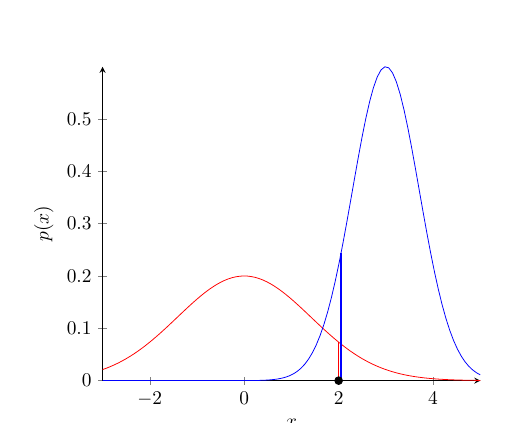
\begin{tikzpicture}[scale=0.7]
\begin{axis}[
    axis lines = left,
    xlabel = \(x\),
    ylabel = {\(p(x)\)},
]
\addplot [
    domain=-3:5, 
    samples=100, 
    color=red,
]
{0.4* 1/2 * exp(-(x^2/4)) };
\addplot [
    domain=-3:5, 
    samples=100, 
    color=blue,
]
{0.6* 1 * exp(-((x-3)^2)) };
\addplot[color=blue,thick] coordinates { (2.05,0) (2.05,0.243) };
\addplot[color=red,thick] coordinates { (2.0,0) (2,0.073) };
\addplot[mark=*] coordinates {(2,0)};
\end{axis}
\end{tikzpicture}
\caption{computing responsibility probabilities; red and blue each indicate their own unnormalized responsibilities}
\end{center}
\end{figure}


\begin{equation}\begin{split}
p (l | x_i, \Theta^{(g)}) = \frac{\alpha_l \N(\x_i | \mu_l, \Sigma_l) }{\sum_{s=1}^k \alpha_s \N(\x_i| \mu_s, \Sigma_s) }
\end{split}\end{equation}


Eq.(\ref{eq M-Step objective function}) shows that the first term contains only $\alpha$ and the second term contains only $\mu, \Sigma$. So we can maximize both terms independently.

%-------------------------------------------------------------

\subsection{The M-Step: maximizing $\alpha$}

Maximizing $\alpha$ means that:

\begin{equation}
\begin{split}
\frac{\partial \sum_{l=1}^k  \sum_{i=1}^{n}  \log ( \alpha_{l}) p(l|x_i,\Theta^{(g)}) }
{\partial \alpha_1, \dots, \partial \alpha_k} = [ 0 \dots 0 ] \hspace{5 mm} \text{subject to } \sum_{l=1}^k \alpha_l = 1\\
\end{split}
\end{equation}

This is to be solved using Lagrange Multiplier

\begin{equation}\begin{split}
&\mathbb{LM}(\alpha_1,\dots \alpha_k, \lambda) =  \sum_{l=1}^k \log ( \alpha_{l}) \underbrace{\bigg( \sum_{i=1}^{n}   p(l|x_i,\Theta^{(g)}) \bigg)}_{\text{contains no } \alpha} + \lambda \bigg(\sum_{l=1}^k \alpha_l  -1  \bigg)\\
\end{split}\end{equation}

taking derivative with respect to just one $\alpha_l$:

\begin{equation}\begin{split}\label{eq Lagrange Multiplier derivative alpha}
\frac{\partial \mathbb{LM}}{\partial \alpha_l} &= \frac{1}{\alpha_l} \bigg( \sum_{i=1}^{n}   p(l|x_i,\Theta^{(g)}) \bigg) + \lambda = 0\\
\implies -\lambda &= \frac{1}{\alpha_l} \bigg( \sum_{i=1}^{n}   p(l|x_i,\Theta^{(g)}) \bigg)\\
\implies -\lambda  \alpha_l &= \bigg( \sum_{i=1}^{n}   p(l|x_i,\Theta^{(g)}) \bigg)\\
\implies -\lambda\sum_{l=1}^k \alpha_l &=\sum_{l=1}^k   \bigg( \sum_{i=1}^{n}   p(l|x_i,\Theta^{(g)}) \bigg)\\
\implies \lambda  &= - n\\
\end{split}\end{equation}

substitute $\lambda  = - n$ into Eq.(\ref{eq Lagrange Multiplier derivative alpha}):

\begin{equation}\begin{split}
\frac{1}{\alpha_l} \bigg( \sum_{i=1}^{n}   p(l|x_i,\Theta^{(g)}) \bigg) + \lambda &= 0\\
\implies \frac{1}{\alpha_l} \bigg( \sum_{i=1}^{n}   p(l|x_i,\Theta^{(g)}) \bigg) -n &= 0\\
\implies \alpha_l &= \frac{1}{n} \sum_{i=1}^{n}   p(l|x_i,\Theta^{(g)}) 
\end{split}\end{equation}


%-------------------------------------------------------------

\subsection{The M-Step: maximizing $\mu, \Sigma$}

Here I jot down the MLE steps for the parameters of a single multidimensional Gaussian distribution. The MLE of a single 1D Gaussian distribution can be easily found in your previous work.

So, maximizing $\mu, \Sigma$ means that:

\begin{equation}
\begin{split}
\frac{\partial \sum_{l=1}^k  \sum_{i=1}^{n}  \log [\mathcal{N}(x_i | \mu_{l}, \Sigma_{l} )] p(l|x_i,\Theta^{(g)}) }
{\partial \mu_1, \dots, \partial \mu_k, \partial \Sigma_1, \dots, \partial \Sigma_k } = [ 0 \dots 0 ] \hspace{5 mm}\\
\end{split}
\end{equation}

You will need some linear algebra identities to solve this; it is quite involved. For full details, refer to Bilmes' gentle tutorial \cite{bilmes1998gentle}.




%-------------------------------------------------------------

\subsubsection{Some formulas to remember}




\begin{itemize}

%\item fact 1:
%
%\begin{equation}
%\begin{split}
%\sum_{i} x_i^T A x_i = \text{tr} \left( A \sum_{i} x_i x_i^T \right)
%\end{split}
%\end{equation}

%\item derivatives of log of determinant ({\color{blue} \bf without} determinant)
%
%\begin{equation}
%\begin{split}
%\frac{\partial \log \X }{\partial \X} = 2 \X^{-1} - \text{diag}(\X^{-1})
%\end{split}
%\end{equation}

\item derivatives of log of determinant ({\color{blue} \bf with} determinant)

\begin{equation}
\begin{split}
\frac{\partial \log | \X | }{\partial \X} = (\X^{-1})^\top 
\end{split}
\end{equation}

\item Derivatives of Traces

\begin{equation}
\begin{split}
\frac{\partial \tr(F(\X)) }{\partial \X} = (f(\X))^\top
\end{split}
\end{equation}

\hspace{10 mm} where $f(\cdot)$ is the {\color{red} scalar derivative} of $F(\cdot)$


\item Derivatives of Traces, fact 1

\begin{equation}
\begin{split}
\frac{\partial \tr( {\bf A} \X  {\bf B}  ) }{\partial \X} = \A^\top \B^\top
\end{split}
\end{equation}

\item Derivatives of Traces of inverse, fact 2

\begin{equation}\begin{split}
\frac{\partial \tr( (\X + \A)^{-1} ) }{\partial \X} = - \big(  (\X + \A)^{-1}  (\X + \A)^{-1} \big)^\top
\end{split}\end{equation}


\item Derivatives of Traces of inverse, fact 3

\begin{equation}
\begin{split}
\frac{\partial \tr( {\bf A} \X^{-1}  {\bf B}  ) }{\partial \X} = -( {\X}^{-1}  {\bf B}  {\bf A} {\X}^{-1}    )^\top
\end{split}
\end{equation}


%When matrix $X$ is symmetric:
%
%\begin{equation}
%\begin{split}
%\frac{\partial \text{tr} ( X B) }{\partial X} = B + B^T - \text{diag}(B)
%\end{split}
%\end{equation}
%
%However, in general:
%
%\begin{equation}
%\begin{split}
%\frac{\partial \text{tr} ( X B) }{\partial X} = B^T
%\end{split}
%\end{equation}

\end{itemize}





%-------------------------------------------------------------

\subsubsection{Maximization $\mu_l$}




\begin{equation}
\begin{split}
\text{second part of } q(\Theta, \Theta^{(g)})
&=  \sum_{l=1}^k  \sum_{i=1}^{n} \log [\mathcal{N}(x_i | \mu_{l}, \SIGMA_{l} ) ] p(l|x_i,\Theta^{(g)})\\
&=  \sum_{i=1}^{n} \sum_{l=1}^k \log \left(  \frac{1}{\sqrt {(2\pi )^{d}|{ \SIGMA_l}|}}  {\exp \bigg(-{\frac {1}{2}}( x_i - \MU_l)^\top \SIGMA_l^{-1}(x_i - \MU_l)\bigg)} \right) p(l|x_i,\Theta^{(g)})\\
\end{split}
\end{equation}


As a template, recall the log-likelihood of $N$ i.i.d.\ zero-meaned columns $\Y$ (each column in $\mathbb{R}^D$) under $\N({\bf 0}, \K)$:

\begin{equation}
\begin{split}
\L \equiv \L(p(\Y| \K)) &= - \frac{D N }{2} \log(2 \pi)  - \frac{N}{2} \log | \K | - \frac{1}{2}  \tr \big( \K^{-1} \Y {\Y}^\top \big)\\
\end{split}
\end{equation}


Let $\Y$ be the zero-meaned data matrix, where each {\color{blue} column} of $\Y$ is $\x_i - \MU_l$:

\begin{equation}
\begin{split}
\mathcal{S}(\mu_{\color{red} l},  \SIGMA_{\color{red} l})
&=   \sum_{i=1}^{n}  -\frac{1}{2} \log ( | \SIGMA_l | ) p(l|x_i,\Theta^{(g)})  -  \sum_{i=1}^{n}  \frac{1}{2}  ( x_i - \MU_l)^\top \SIGMA_l^{-1} (x_i - \MU_l)  p(l|x_i,\Theta^{(g)}) + \C\\
\end{split}
\end{equation}



\begin{equation}
\begin{split}
\implies \mathcal{S}(\mu_l, \Sigma_l^{-1})  &=   - \tr \left( \frac{\Sigma_l^{-1}}{2} \sum_{i=1}^{n}  ( x_i - \mu_l)  (x_i - \mu_l)^\top p(l|x_i,\Theta^{(g)})   \right)   + \text{ Constant} \\
%----------------------------------------------------------
\implies  \frac{\partial \mathcal{S}(\mu_l, \Sigma_l^{-1})}{\partial \mu_l} &=   \frac{\Sigma_l^{-1} }{2} \sum_{i=1}^{n}   2  ( x_i - \mu_l) p(l|x_i,\Theta^{(g)}) = 0\\
%----------------------------------------------------------
\implies  \sum_{i=1}^{n}  x_i  p(l|x_i,\Theta^{(g)})  &= \mu_l  \sum_{i=1}^{n}  p(l|x_i,\Theta^{(g)})   \\
%----------------------------------------------------------
\implies   \mu_l &=  \frac{ \sum_{i=1}^{n}  x_i  p(l|x_i,\Theta^{(g)})} { \sum_{i=1}^{n}  p(l|x_i,\Theta^{(g)}) }  \\
\end{split}
\end{equation}








%-------------------------------------------------------------

\subsubsection{Maximization of covariance}

\begin{equation}
\begin{split}
\text{second part of } q(\Theta, \Theta^{(g)})
&=  \sum_{l=1}^k  \sum_{i=1}^{n} \log [\mathcal{N}(x_i | \mu_{l}, \SIGMA_{l} ) ] p(l|x_i,\Theta^{(g)})\\
&=  \sum_{i=1}^{n} \sum_{l=1}^k \log \left(  \frac{1}{\sqrt {(2\pi )^{d}|{ \SIGMA_l}|}}  {\exp \bigg(-{\frac {1}{2}}( x_i - \MU_l )^\top \SIGMA_l^{-1}(x_i - \MU_l )\bigg)} \right) p(l|x_i,\Theta^{(g)})\\
%\implies \mathcal{S}(\mu_{\color{red} l},  \SIGMA_{\color{red} l}) 
%&=   \sum_{i=1}^{n}  -\frac{1}{2} \log ( | \SIGMA_l | ) p(l|x_i,\Theta^{(g)})  -  \sum_{i=1}^{n}  \frac{1}{2}  ( x_i - \MU_l)^T \SIGMA^{-1} (x- \MU_l)  p(l|x_i,\Theta^{(g)})\\
\end{split}
\end{equation}

\begin{itemize}
\item
let $\Y$ be zero-meaned data matrix, where each {\color{blue} column} of $\Y$ is $x_i - \MU_l$
\item
let $\P$ be diagonal matrix in which $\P_{ii}$ correspond to $p( l | x_i,\Theta^{(g)})$
\end{itemize}

\begin{equation}
\begin{split}
\L \equiv \L(p(\Y| \MU_l, \SIGMA_l)) &= - \frac{d \times \tr(\P) }{2} \log(2 \pi)  - \frac{\tr(\P)}{2} \log | \SIGMA_l | - \frac{1}{2}  \tr \big( \SIGMA_l^{-1} \Y \P {\Y}^\top \big)\\
\end{split}
\end{equation}



%\begin{equation}
%\begin{split}
%\text{second part of } q(\Theta, \Theta^{(g)})
%&=  \sum_{l=1}^k  \sum_{i=1}^{n} \log [\mathcal{N}(x_i | \mu_{l}, \SIGMA_{l} ) ] p(l|x_i,\Theta^{(g)})\\
%&=  \sum_{i=1}^{n} \sum_{l=1}^k \log \left(  \frac{1}{\sqrt {(2\pi )^{d}|{ \SIGMA_l}|}}  {\exp \bigg(-{\frac {1}{2}}( x_i -{\boldsymbol {\mu }})^\top \SIGMA^{-1}(x_i -{\boldsymbol {\mu }})\bigg)} \right) p(l|x_i,\Theta^{(g)})\\
%\implies \mathcal{S}(\mu_{\color{red} l},  \SIGMA_{\color{red} l}) 
%&=   \sum_{i=1}^{n}  -\frac{1}{2} \log ( | \SIGMA_l | ) p(l|x_i,\Theta^{(g)})  -  \sum_{i=1}^{n}  \frac{1}{2}  ( x_i - \MU_l)^T \SIGMA^{-1} (x- \MU_l)  p(l|x_i,\Theta^{(g)})\\
%\end{split}
%\end{equation}


\begin{equation}
\begin{split}
\frac{\partial \L}{ \partial \SIGMA_l} &=  
 {\SIGMA_l}^{-1}  \Y \P \Y^\top \SIGMA_l^{-1} - \tr(\P)  \SIGMA_l^{-1} = {\bf 0}  \\
%  ( {\SIGMA_l}^{-1}  \Y) ( \SIGMA_l^{-1} \Y)^\top - D \SIGMA_l^{-1} = {\bf 0} \\
\implies  {\SIGMA_l}^{-1}  \Y \P \Y^\top \SIGMA_l^{-1}  &=  \tr(\P)  \SIGMA_l^{-1} \\
\implies  \Y \P \Y^\top  \SIGMA_l^{-1}  &=  \tr(\P) \, \I \\
\implies  \SIGMA_l^{-1}  &=  \tr(\P)  (\Y \P \Y^\top)^{-1}  \\
\implies  \SIGMA_l  &=  \tr(\P)^{-1}  (\Y \P \Y^\top)
=  \frac{(\Y \P \Y^\top)}{\tr(\P) }\\
 &=  \frac{\sum_{i=1}^{n}  ( x_i - \mu_l) (x_i - \mu_l)^\top p(l | x_i,\Theta^{(g)})}{ \sum_{i=1}^{n} p(l | x_i,\Theta^{(g)})} \\
\end{split}
\end{equation}



%\begin{equation}
%\begin{split}
%\implies \mathcal{S}(\mu_l, \Sigma_l^{-1})  &=   - \text{Tr} \left( \frac{\Sigma_l^{-1}}{2} \sum_{i=1}^{n}  ( x_i - \mu_l)  (x_i - \mu_l)^T p(l|x_i,\Theta^{(g)})   \right)   + \text{ Constant} \\
%%----------------------------------------------------------
%\implies  \frac{\partial \mathcal{S}(\mu_l, \Sigma_l^{-1})}{\partial \mu_l} &=   \frac{\Sigma^{-1} }{2} \sum_{i=1}^{n}   2  ( x_i - \mu_l) p(l|x_i,\Theta^{(g)}) = 0\\
%%----------------------------------------------------------
%\implies  \sum_{i=1}^{n}  x_i  p(l|x_i,\Theta^{(g)})  &= \mu_l  \sum_{i=1}^{n}  p(l|x_i,\Theta^{(g)})   \\
%%----------------------------------------------------------
%\implies   \mu_l &=  \frac{ \sum_{i=1}^{n}  x_i  p(l|x_i,\Theta^{(g)})} { \sum_{i=1}^{n}  p(l|x_i,\Theta^{(g)}) }  \\
%\end{split}
%\end{equation}


%-------------------------------------------------------------

%\subsection{Maximization $\Sigma_l$}

\begin{equation}
\begin{split}
 \mathcal{S}(\mu_l, \Sigma_l^{-1}) &=   \sum_{i=1}^{n}   \left(  -\frac{1}{2} \log ( | \Sigma_l | )  -\frac{1}{2} ( x_i - \mu_l)^\top \Sigma_l^{-1} (x_i - \mu_l) \right)  p(l|x_i,\Theta^{(g)})\\
\end{split}
\end{equation}

Change $\Sigma$ to $\Sigma^{-1}$, this is so that after taking derivative of $\log (X) $, the result is in terms of $X^{-1}$

\begin{equation}\begin{split}
 &=    \Bigg(  \frac{1}{2} \sum_{i=1}^{n}  \log ( | \Sigma_l^{-1} | )  p(l|x_i,\Theta^{(g)})  -\frac{1}{2} \text{tr} \Bigg( \Sigma_l^{-1} \underbrace{\sum_{i=1}^{n}  ( x_i - \mu_l) (x_i - \mu_l)^\top  p(l|x_i,\Theta^{(g)}) }_{M_l} \Bigg) \Bigg) \\
%------------------------------------------------------------
\implies  \frac{\partial \mathcal{S}(\mu_l, \Sigma_l^{-1})}{\partial \Sigma^{-1}_l} &=     \frac{2   \sum_{i=1}^{n} \Sigma_l p(l|x_i,\Theta^{(g)}) -  \sum_{i=1}^{n} \text{diag}(\Sigma_l) p(l|x_i,\Theta^{(g)}) }{2}    -\frac{2M_l - \text{diag}(M_l)}{2} = 0 \\
%------------------------------------------------------------
\implies & 2 \Big(  \sum_{i=1}^{n} \Sigma_l p(l | x_i,\Theta^{(g)}) - M_l \Big)   -  \text{diag} \Big( \sum_{i=1}^{n} \Sigma_l p(l | x_i,\Theta^{(g)}) - M_l \Big)   = 0\\
%------------------------------------------------------------
\implies & \sum_{i=1}^{n} \Sigma_l p(l | x_i,\Theta^{(g)}) - M_l = 0\\
\implies & \Sigma_l = \frac{M_l}{\sum_{i=1}^{n} p(l | x_i,\Theta^{(g)})} =  \frac{\sum_{i=1}^{n}  ( x_i - \mu_l) (x_i - \mu_l)^\top p(l | x_i,\Theta^{(g)})}{ \sum_{i=1}^{n} p(l | x_i,\Theta^{(g)})}
\end{split}\end{equation}







%-------------------------------------------------------------

\subsection{Summary of Gaussian Mixture Model}

In summary, to update $\Theta^{(g)} \rightarrow \Theta^{(g+1)}$:

\begin{equation}\begin{split}
\alpha_l^{(g+1)} = \frac{1}{n} \sum_{i=1}^n p (l | x_i, \Theta^{(g)})
\end{split}\end{equation}

\begin{equation}\begin{split}
\mu_l^{(g+1)} = \frac{\sum_{i=1}^n x_i p (l | x_i, \Theta^{(g)})}{\sum_{i=1}^n p (l | x_i, \Theta^{(g)})}
\end{split}\end{equation}

\begin{equation}\begin{split}
\Sigma_l^{(g+1)} = \frac{\sum_{i=1}^n [x_i - \mu_l^{(g+1)}] [ x_i - \mu_l^{(g+1)} ]^\top p (l | x_i, \Theta^{(g)})}{\sum_{i=1}^n p (l | x_i, \Theta^{(g)})}
\end{split}\end{equation}

One can verify that when the number of components $k = 1 \implies p (l=1 | x_i, \Theta^{(g)}) = 1$, then:

\begin{equation}\begin{split}
\alpha_l^{(g+1)} = 1
\end{split}\end{equation}

\begin{equation}\begin{split}
\mu_l^{(g+1)} = \frac{1}{n }\sum_{i=1}^n x_i
\end{split}\end{equation}

\begin{equation}\begin{split}
\Sigma_l^{(g+1)} = \frac{1}{n} \sum_{i=1}^n [x_i - \mu_l^{(g+1)}] [ x_i - \mu_l^{(g+1)} ]^\top
\end{split}\end{equation}

which becomes the parameter update of a single Gaussian

%To program it to MATLAB, note that we need to compute the responsibility probability $p (l | x_i, \Theta^{(g)}) = \frac{\mathcal{N}(x_i | \mu_l, \Sigma_l) }{\sum_{s=1}^k \mathcal{N}(x_i| \mu_s, \Sigma_s) }$ 



%-------------------------------------------------------------

\subsection{GMM fitting: initialization vs.\ convergence}

\begin{figure}[H]
     \centering
     \begin{subfigure}[b]{0.48\textwidth}
         \centering
         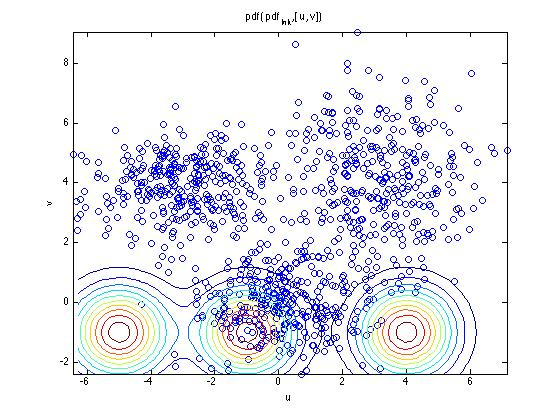
\includegraphics[width=\textwidth]{gmm_init_3_mixtures.jpg}
         \caption{GMM at initialization: $\Theta^{(1)}$}
     \end{subfigure}
     \begin{subfigure}[b]{0.48\textwidth}
         \centering
         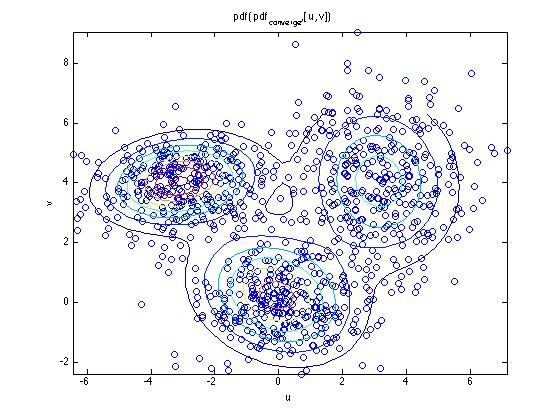
\includegraphics[width=\textwidth]{gmm_result_3_mixtures.jpg}
         \caption{GMM at convergence: $\Theta^{(\text{final})}$}
     \end{subfigure}
\end{figure}


%%-------------------------------------------------------------
%
%\subsection{Other clustering methods: K-means}
%
%This shows the data and the initial ``means'':
%\begin{figure}
%    \begin{center}
%    \includegraphics[scale=0.32]{kmeans_init.jpg}
%     \end{center}
%\end{figure}
%
%%-------------------------------------------------------------
%\begin{itemize}
%\item Imagine we know that there are $K$ types of data, and we have $N$ data.
%\item How do we cluster these $N$ data into $K$ types “automatically”?
%\item Like GMM, this is unsupervised, “clustering” algorithm
%\end{itemize}
%
%%-------------------------------------------------------------
%\subsection{K-means Algorithm}
%\begin{itemize}
%\item {\bf STEP 1:} Place $K$ points into the space represented by the objects that are being clustered. These points represent initial group centroids.
%\item {\bf STEP 2:} Assign each object to the group that has the closest centroid.
%\item {\bf STEP 3:} When all objects have been assigned, recalculate the positions of the $K$ centroids. Repeat Steps 2 and 3 until the centroids no longer move.
%\end{itemize}
%
%%-------------------------------------------------------------
%
%\subsection{K-means}
%
%The data and the initial $K$ ``means'':
%\begin{figure}
%    \begin{center}
%    \includegraphics[scale=0.32]{kmeans_init.jpg}
%     \end{center}
%\end{figure}
%
%%-------------------------------------------------------------
%
%The final $K$ ``means'':
%
%\begin{figure}
%    \begin{center}
%    \includegraphics[scale=0.32]{kmeans_result.jpg}
%     \end{center}
%\end{figure}
%See the MATLAB Demos
%%-------------------------------------------------------------

\bibliography{../includes/refs}
\bibliographystyle{../includes/IEEEbib}
\end{document}
